\section{Simplified Environment Results}

All three algorithms successfully converge to a decent grasping policy in the simplified environment. BDQ and DQN  were trained with varying action dimension padding 2, 4, 8, 16, and 33.
We observed how the neural network size affects the success rate. Two different network sizes were tried on BDQ; a large network with two hidden layers in shared module with 512 and 256 neurons each and 128 each for state and advantage function estimators, and a small network with two hidden layers in the shared representation with 64 neurons each and 32 neurons each for the state and advantage function estimators. Furthermore, we compared the BDQ performance with two different buffer sizes, fifty thousand and one million. We did not vary the  DQN's algorithm's hyperparameters. The default buffer size of 50k was used for all trials of DQN.
As for the SAC algorithm, we only change the input from the encoder to depth in the simplified environment.

\begin{table}[!htbp]
    \begin{tabular}{|l|l|l|l|l|}
    \hline
                       & \multicolumn{4}{c|}{\textbf{BDQ Simplified Scenario}}              \\ \hline
                       & \multicolumn{2}{c|}{Floor Scene} & \multicolumn{2}{c|}{Table Scene} \\ \hline
    Models             & Training Set      & Test Set     & Training Set      & Test Set     \\ \hline
    \textbf{BDQ\_33pads\_big}   & 34\%              & 29\%         & 13\%              & 12\%         \\ \hline
    \textbf{BDQ\_33pads\_small} & 90\%              & 82\%         & 86\%              & 79\%         \\ \hline
    \textbf{BDQ\_16pads\_small} & 89\%              & 93\%         & 90\%              & 91\%         \\ \hline
    \textbf{BDQ\_8pads\_small}  & 91\%              & 90\%         & 77\%              & 72\%         \\ \hline
    \textbf{BDQ\_4\_pads}       & 96\%              & 94\%         & 92\%              & 89\%         \\ \hline
    \end{tabular}
    \caption{BDQ algorithm's result in the simplified environment}
\end{table}


\begin{table}[!htbp]
    \begin{tabular}{|l|l|l|l|l|}
    \hline
                         & \multicolumn{4}{c|}{\textbf{DQN Simplified Scenario}}                                 \\ \hline
                         & \multicolumn{2}{c|}{\textbf{Floor Scene}} & \multicolumn{2}{c|}{\textbf{Table Scene}} \\ \hline
    \textbf{Models}      & \textbf{Training Set} & \textbf{Test Set} & \textbf{Training Set} & \textbf{Test Set} \\ \hline
    \textbf{DQN\_33pads} & 6\%                   & 6\%               & 6\%                   & 7\%               \\ \hline
    \textbf{DQN\_16pads} & 12\%                  & 6\%               & 9\%                   & 14\%              \\ \hline
    \textbf{DQN\_8pads}  & 75\%                  & 65\%              & 38\%                  & 40\%              \\ \hline
    \textbf{DQN\_4pads}  & 75\%                  & 73\%              & 1\%                   & 1\%               \\ \hline
    \textbf{DQN\_2pads}  & 76\%                  & 74\%              & 55\%                  & 63\%              \\ \hline
    \end{tabular}
    \caption{DQN algorithm's result in the simplified environment}
\end{table}



\begin{table}[!htbp]
    \begin{tabular}{|l|l|l|l|l|}
    \hline
                                    & \multicolumn{4}{c|}{\textbf{SAC Simplified  Scenario}}                         \\ \hline
                                    & \multicolumn{2}{c|}{\textbf{Floor Scene}} & \multicolumn{2}{c|}{\textbf{Table Scene}} \\ \hline
    \textbf{Models}                 & \textbf{Training Set}   & \textbf{Test Set}  & \textbf{Training Set} & \textbf{Test Set} \\ \hline
    \textbf{SAC\_encoder} & 98\%                 & 97\%               & 84\%                  & 87\%              \\ \hline
    \textbf{SAC\_depth}   & 91\%                 & 96\%               & 28\%                  & 24\%              \\ \hline
    \end{tabular}
    \caption{SAC algorithm's result in the simplified environment}
\end{table}

\begin{figure}[!htbp]
    \begin{subfigure}{0.49\textwidth}
        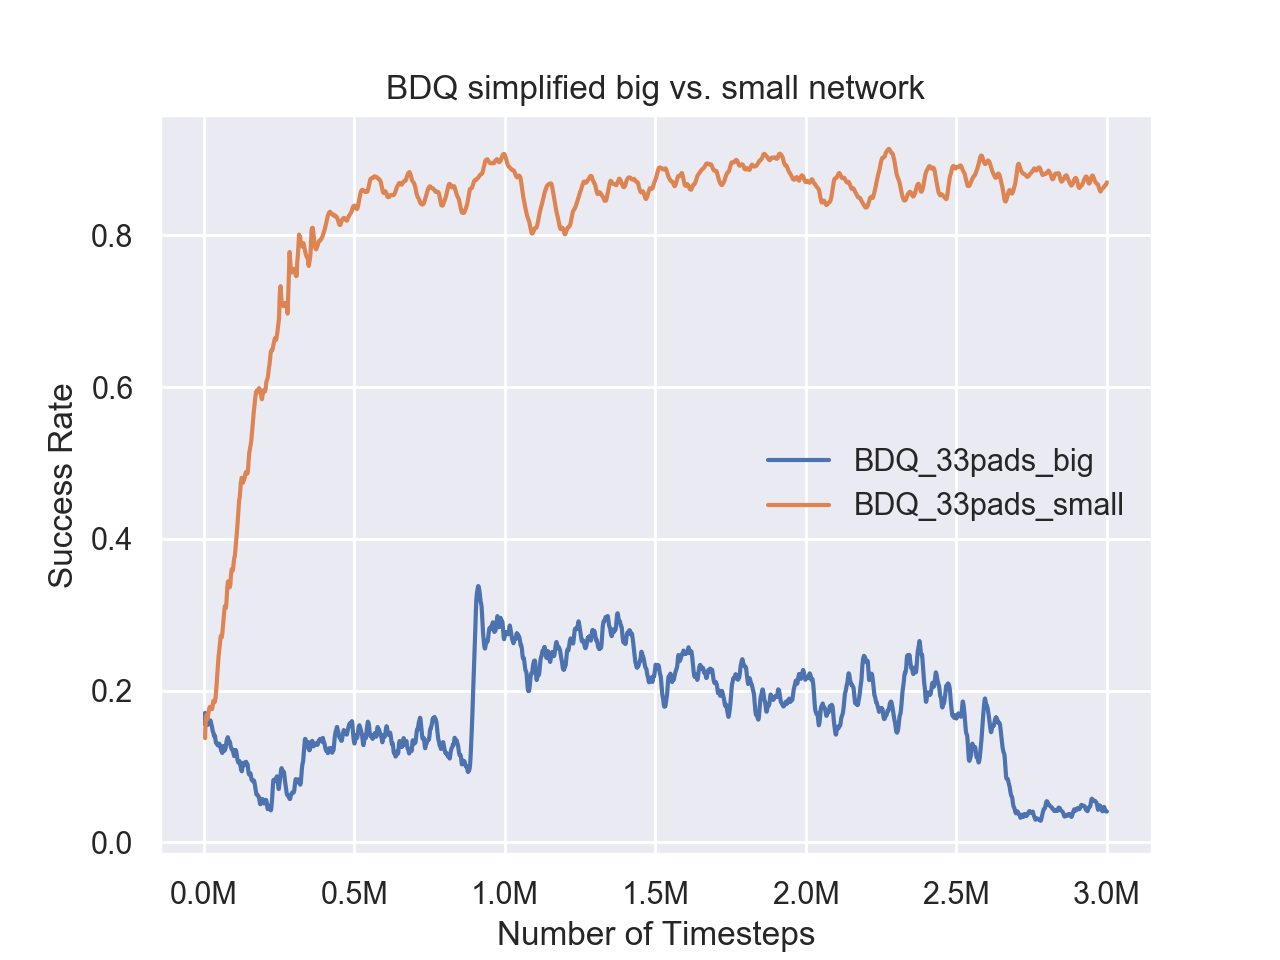
\includegraphics[width=\linewidth]{figures/BDQ_simplified_big_vs_small_network_no_var}
        \caption{Table Scene} \label{fig:table}
    \end{subfigure}%
    \hspace*{\fill}   % maximize separation between the subfigures
    \begin{subfigure}{0.49\textwidth}
        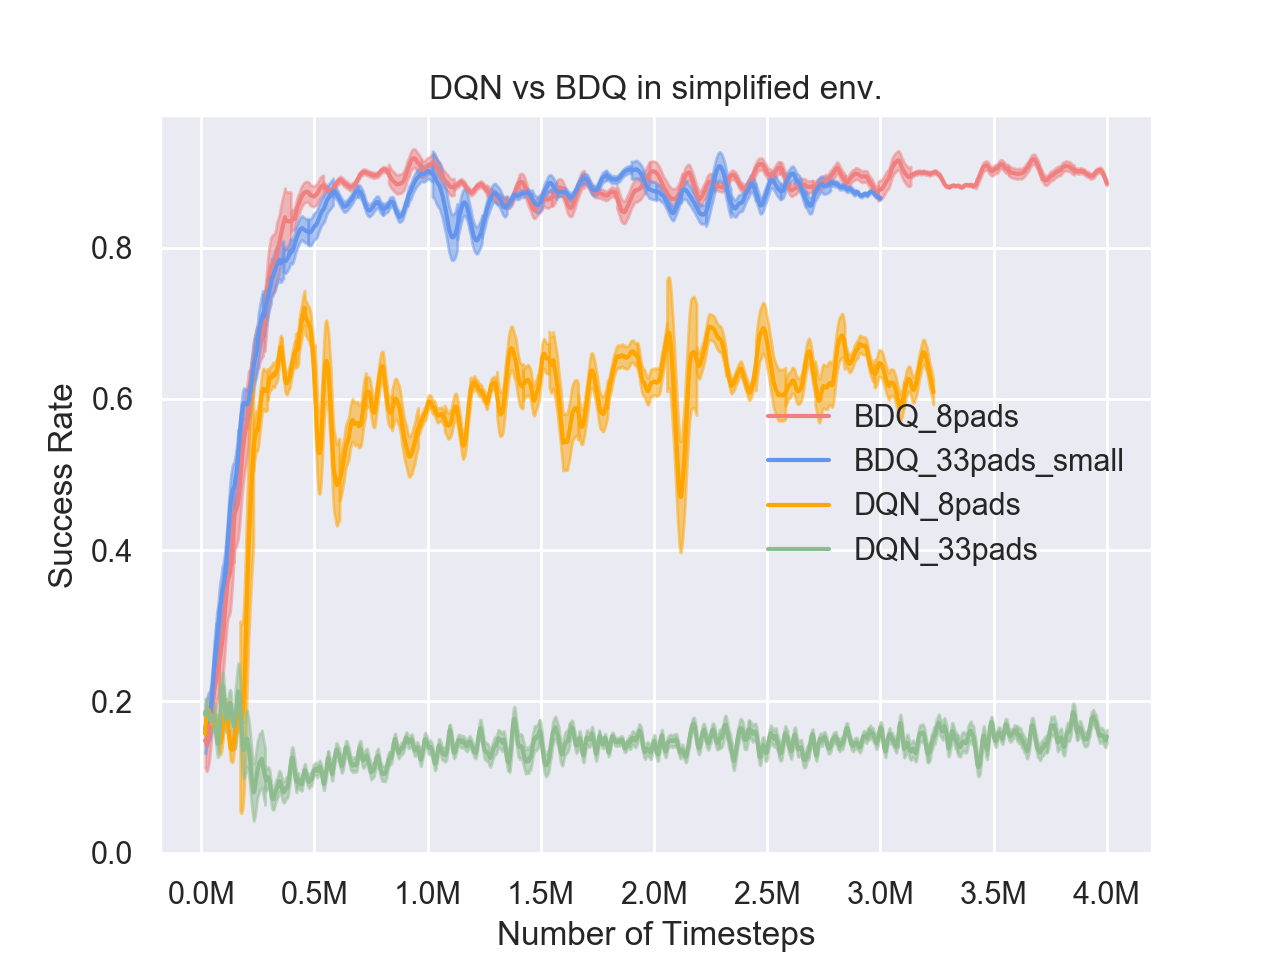
\includegraphics[width=\linewidth]{figures/DQN_vs_BDQ_in_simplified_env}
        \caption{Floor Scene} \label{fig:floor}
    \end{subfigure}%
    \hspace*{\fill}   % maximize separation between the subfigures


\caption{ Table and floor scenes \label{fig:scenes}}
\end{figure}

\begin{figure}[!htbp]
    \begin{subfigure}{0.49\textwidth}
        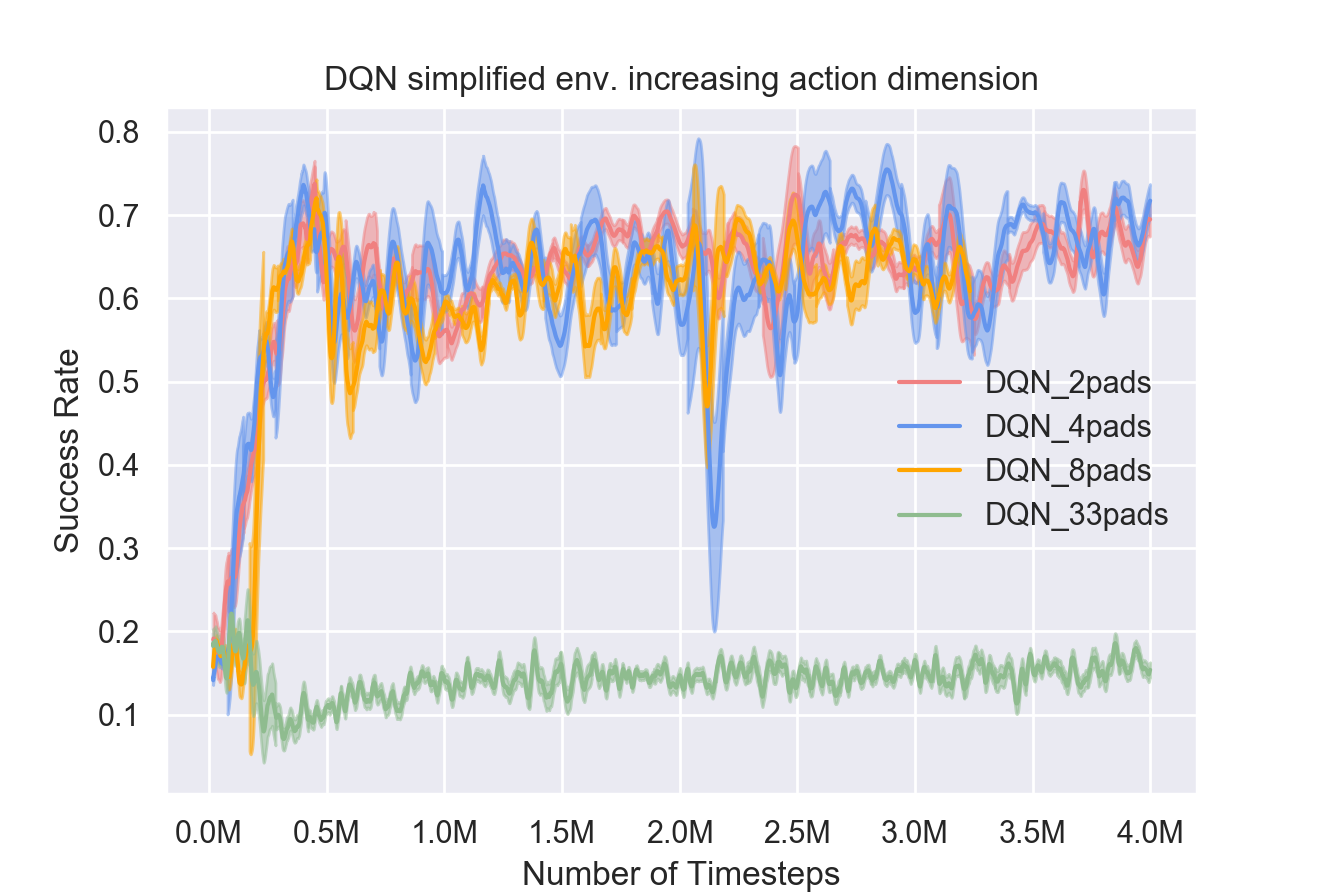
\includegraphics[width=\linewidth]{figures/DQN_simplified_env_increasing_action_dimension}
        \caption{Table Scene} \label{fig:table}
    \end{subfigure}%
    \hspace*{\fill}   % maximize separation between the subfigures
    \begin{subfigure}{0.49\textwidth}
        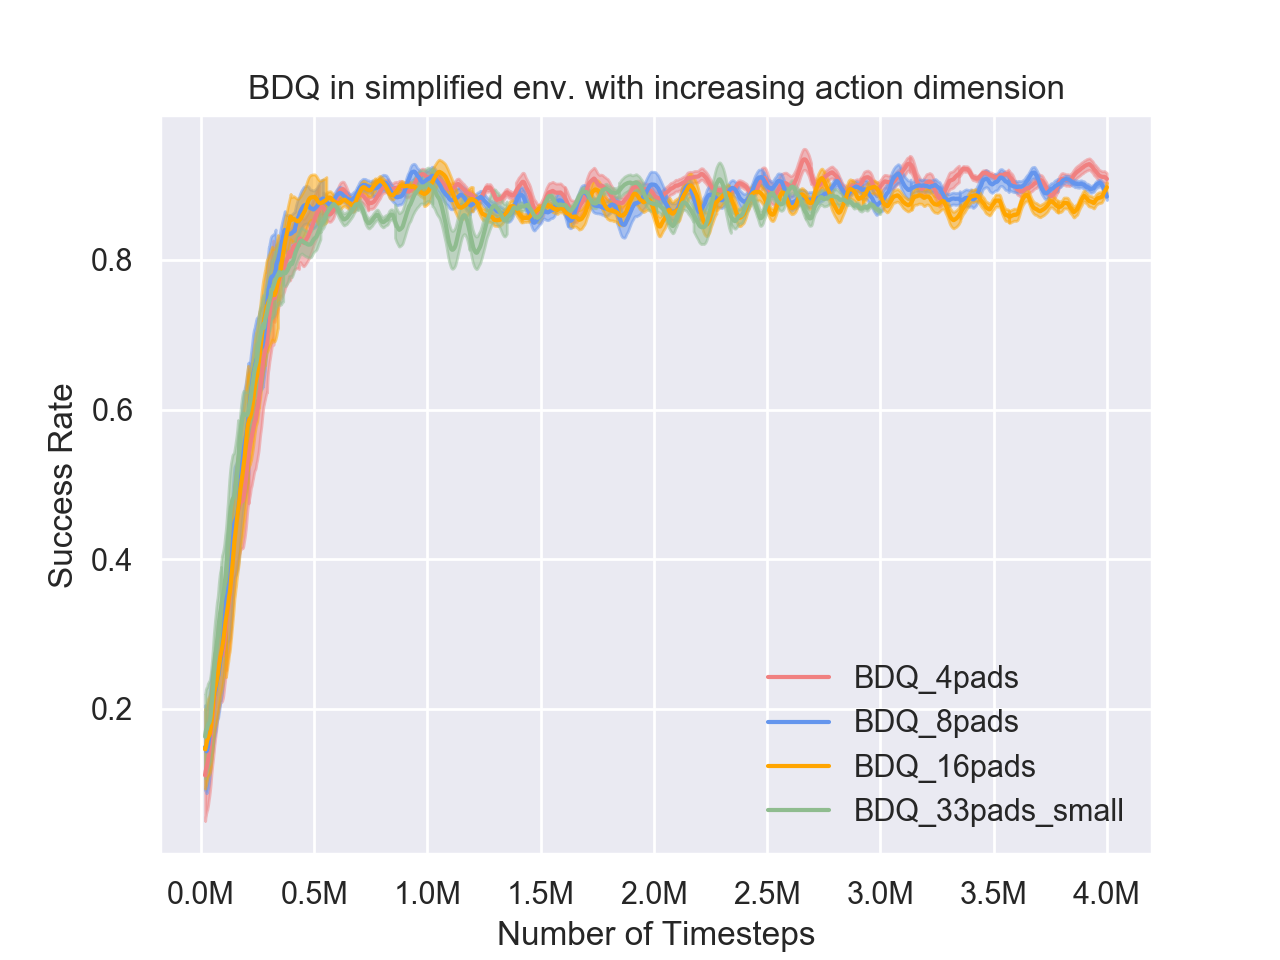
\includegraphics[width=\linewidth]{figures/BDQ_in_simplified_env_with_increasing_action_dimension}
        \caption{Floor Scene} \label{fig:floor}
    \end{subfigure}%
    \hspace*{\fill}   % maximize separation between the subfigures


\caption{ Table and floor scenes \label{fig:scenes}}
\end{figure}



\begin{figure}[!htbp]
    \begin{subfigure}{0.49\textwidth}
        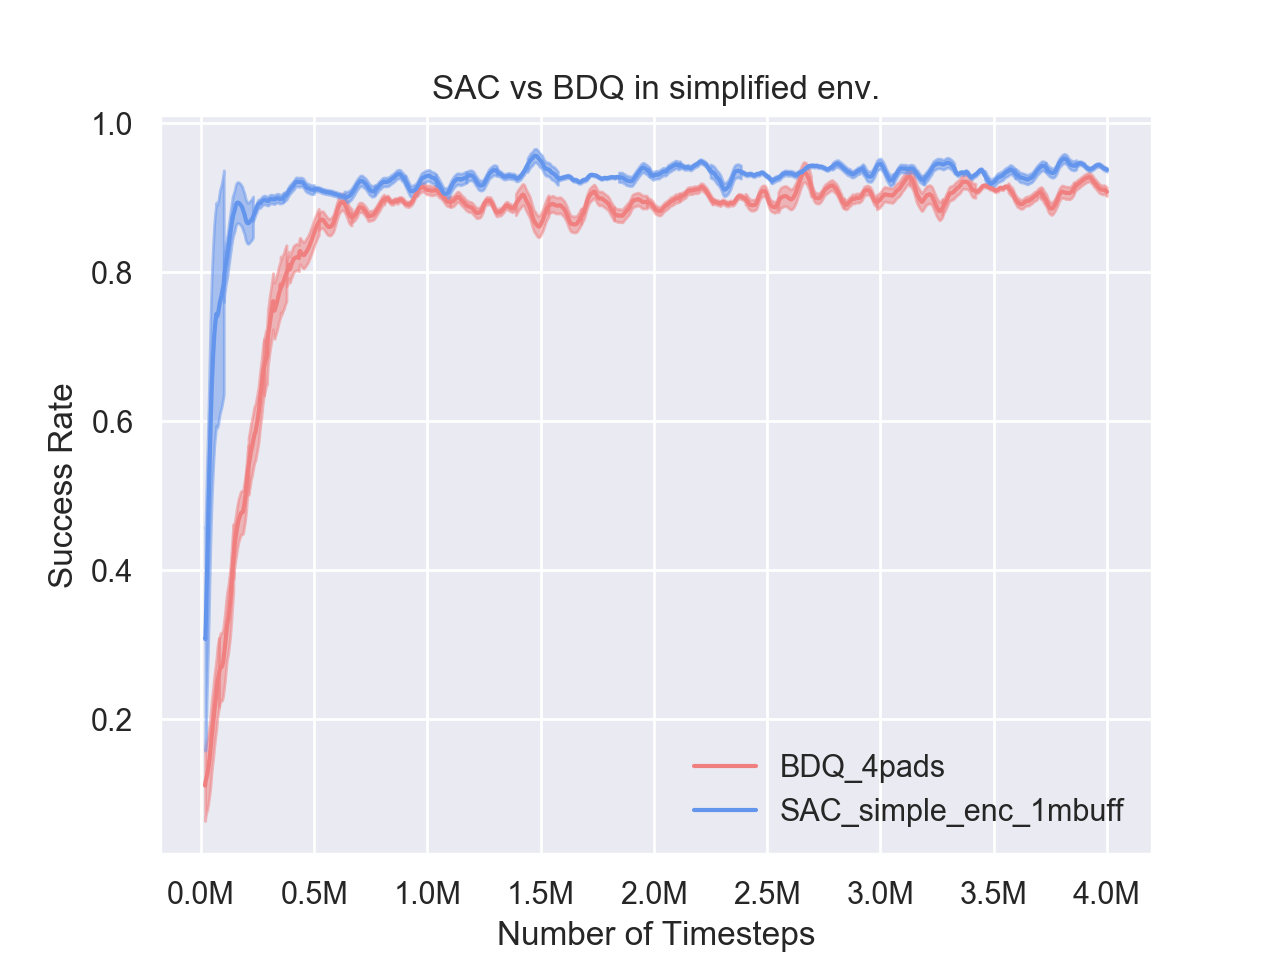
\includegraphics[width=\linewidth]{figures/SAC_vs_BDQ_in_simplified_env}
        \caption{Table Scene} \label{fig:table}
    \end{subfigure}%
    \hspace*{\fill}   % maximize separation between the subfigures
    \begin{subfigure}{0.49\textwidth}
        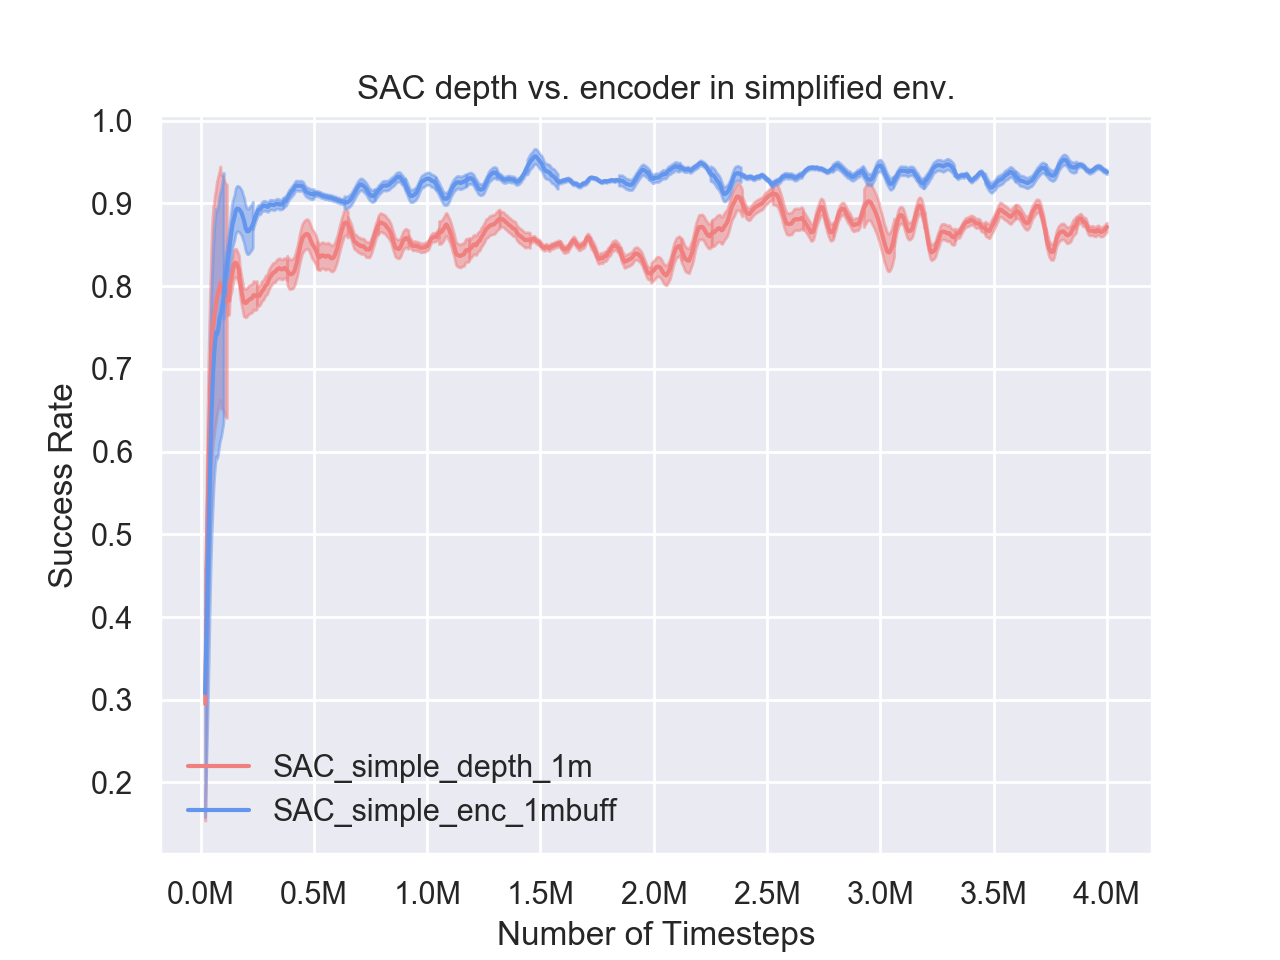
\includegraphics[width=\linewidth]{figures/SAC_depth_vs_encoder_in_simplified_env}
        \caption{Floor Scene} \label{fig:floor}
    \end{subfigure}%
    \hspace*{\fill}   % maximize separation between the subfigures


\caption{ Table and floor scenes \label{fig:scenes}}
\end{figure}

% \begin{figure}[!htbp]
%     \centering
%         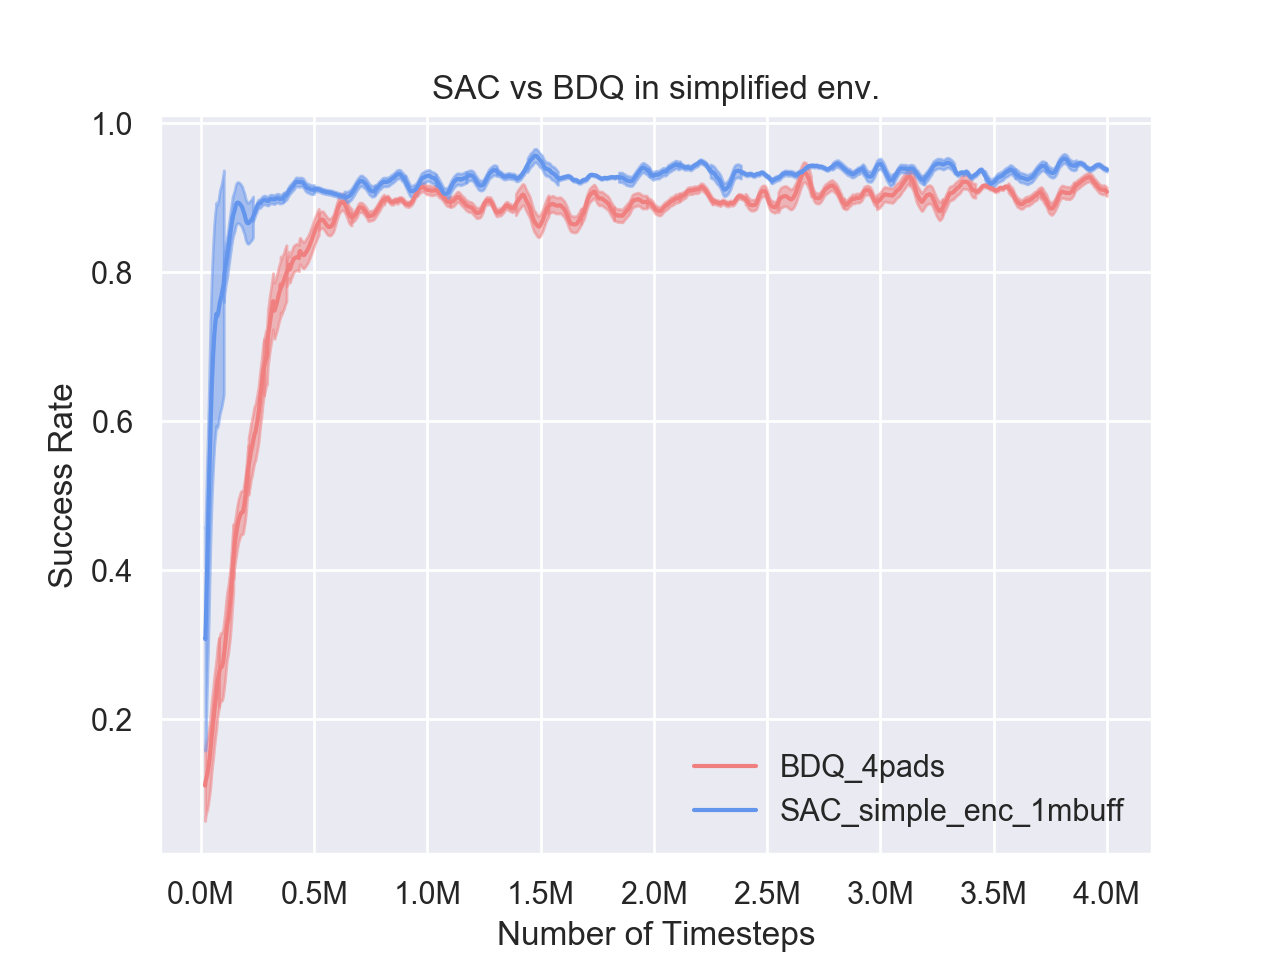
\includegraphics[width=0.4\textwidth]{figures/SAC_vs_BDQ_in_simplified_env}
%     \caption{Different manipulation skill adopted to robotic manipulators \cite{Kroemer2019}}
%     \label{fig:x manipulation_skills}
% \end{figure}

% \begin{figure}[!htbp]
%     \centering
%         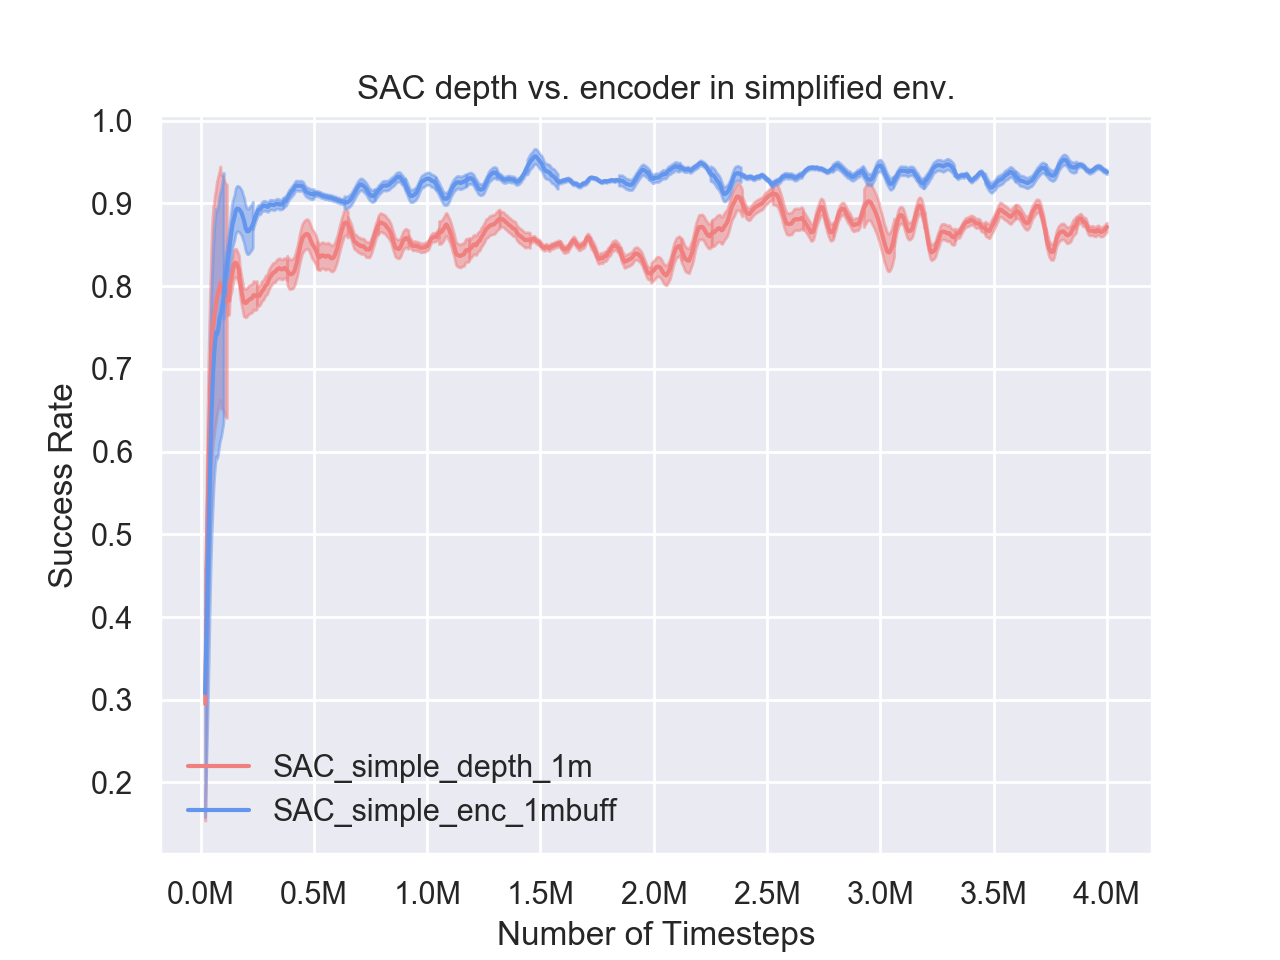
\includegraphics[width=0.4\textwidth]{figures/SAC_depth_vs_encoder_in_simplified_env}
%     \caption{Different manipulation skill adopted to robotic manipulators \cite{Kroemer2019}}
%     \label{fig:x manipulation_skills}
% \end{figure}

